\begin{posterblock}{white}{smucyan}{smunavy}{smuice}{R1. Results: DIC/PLC Mechanism Evidence}
\centering
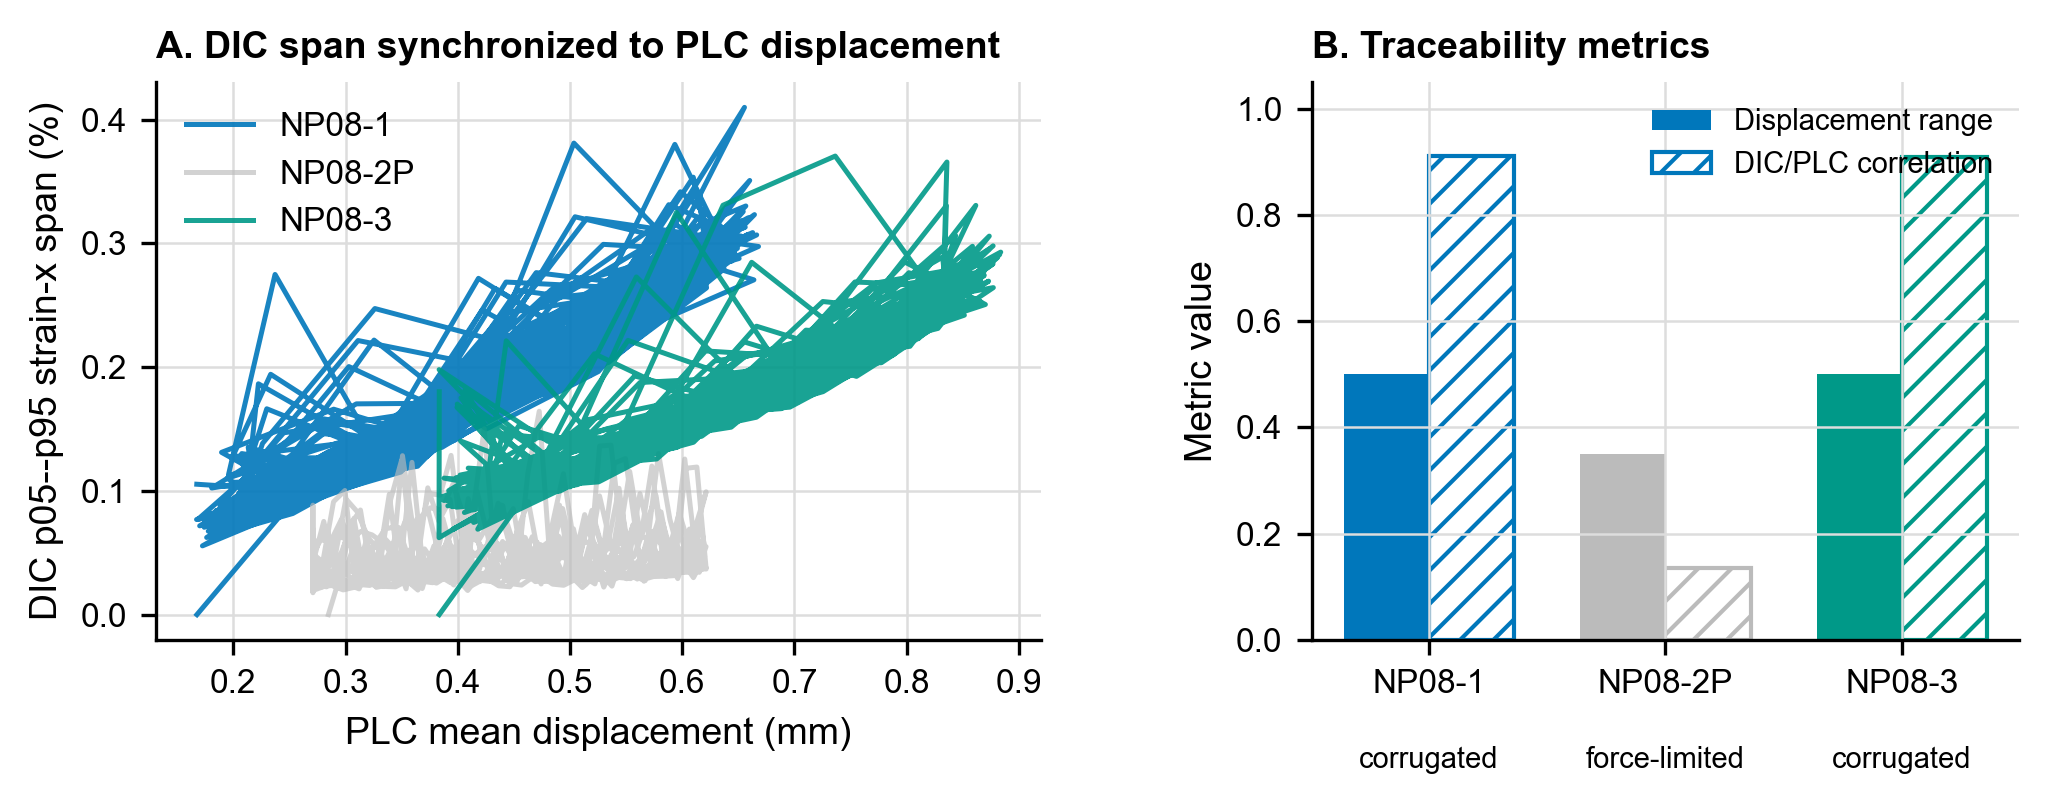
\includegraphics[width=\linewidth,height=15.8cm,keepaspectratio]{assets/fig02_dic_plc_traceability.png}
\smallnote{DIC strain span follows imposed PLC mean displacement.}

\vspace{0.6ex}
\centering
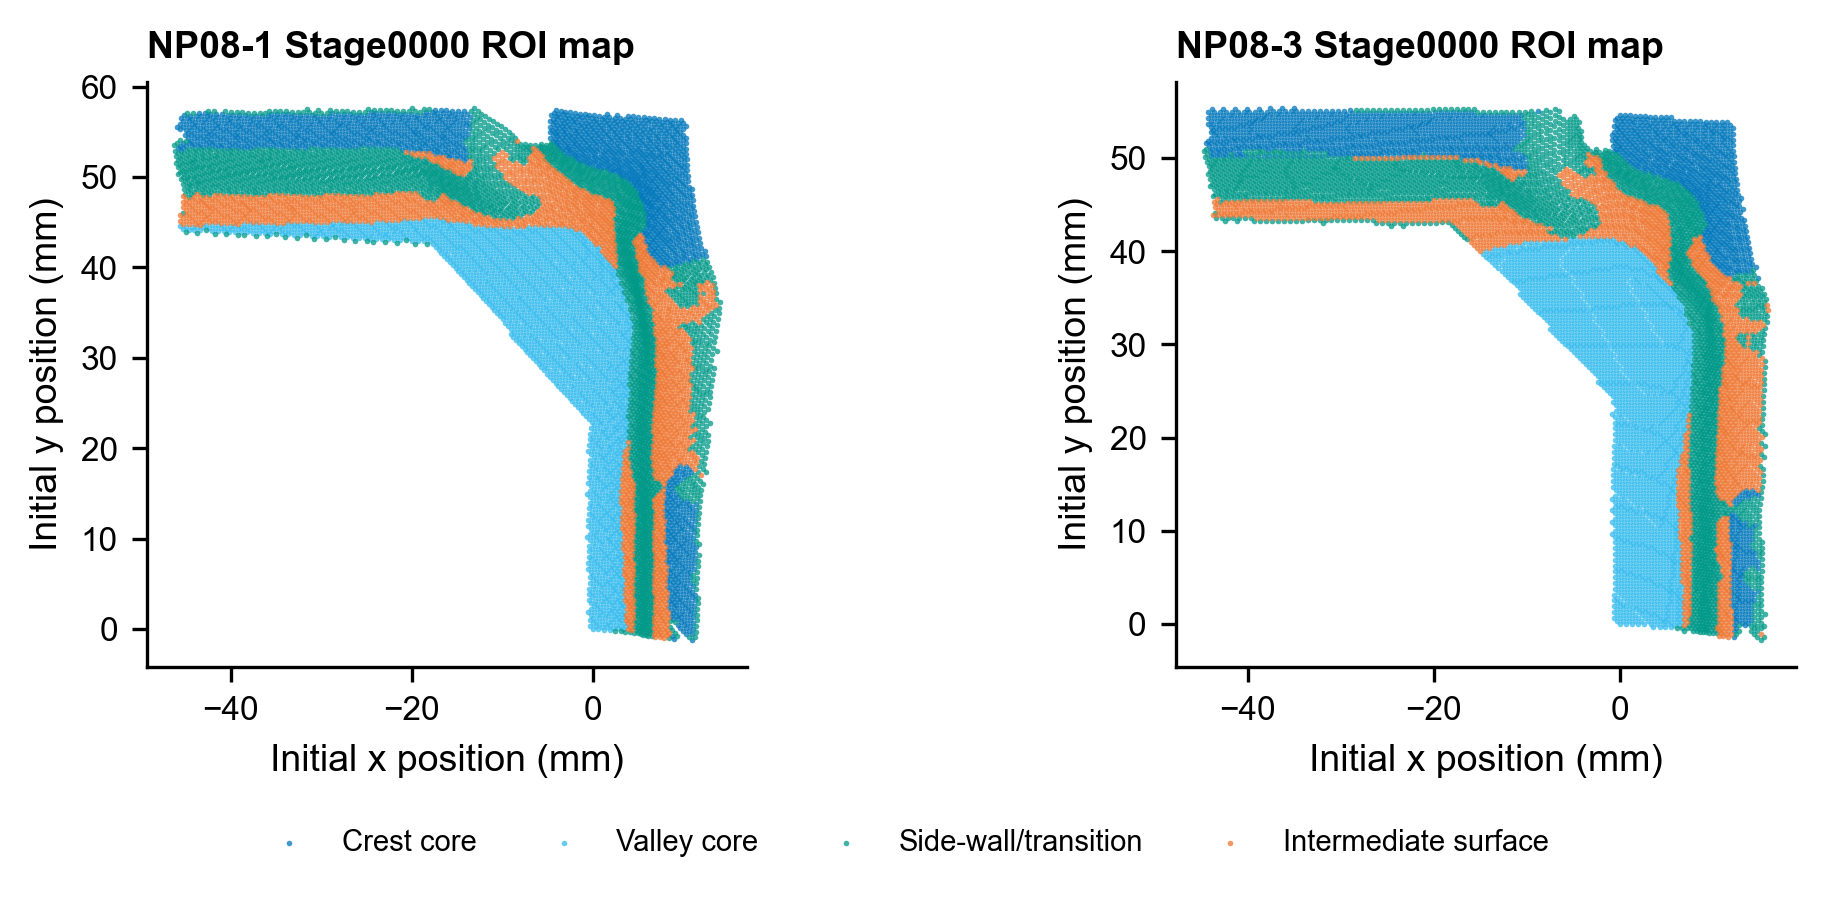
\includegraphics[width=\linewidth,height=18.2cm,keepaspectratio]{assets/fig03_dic_geometry_roi_map.png}
\smallnote{Initial geometry defines persistent ROI labels.}

\vspace{0.6ex}
\centering
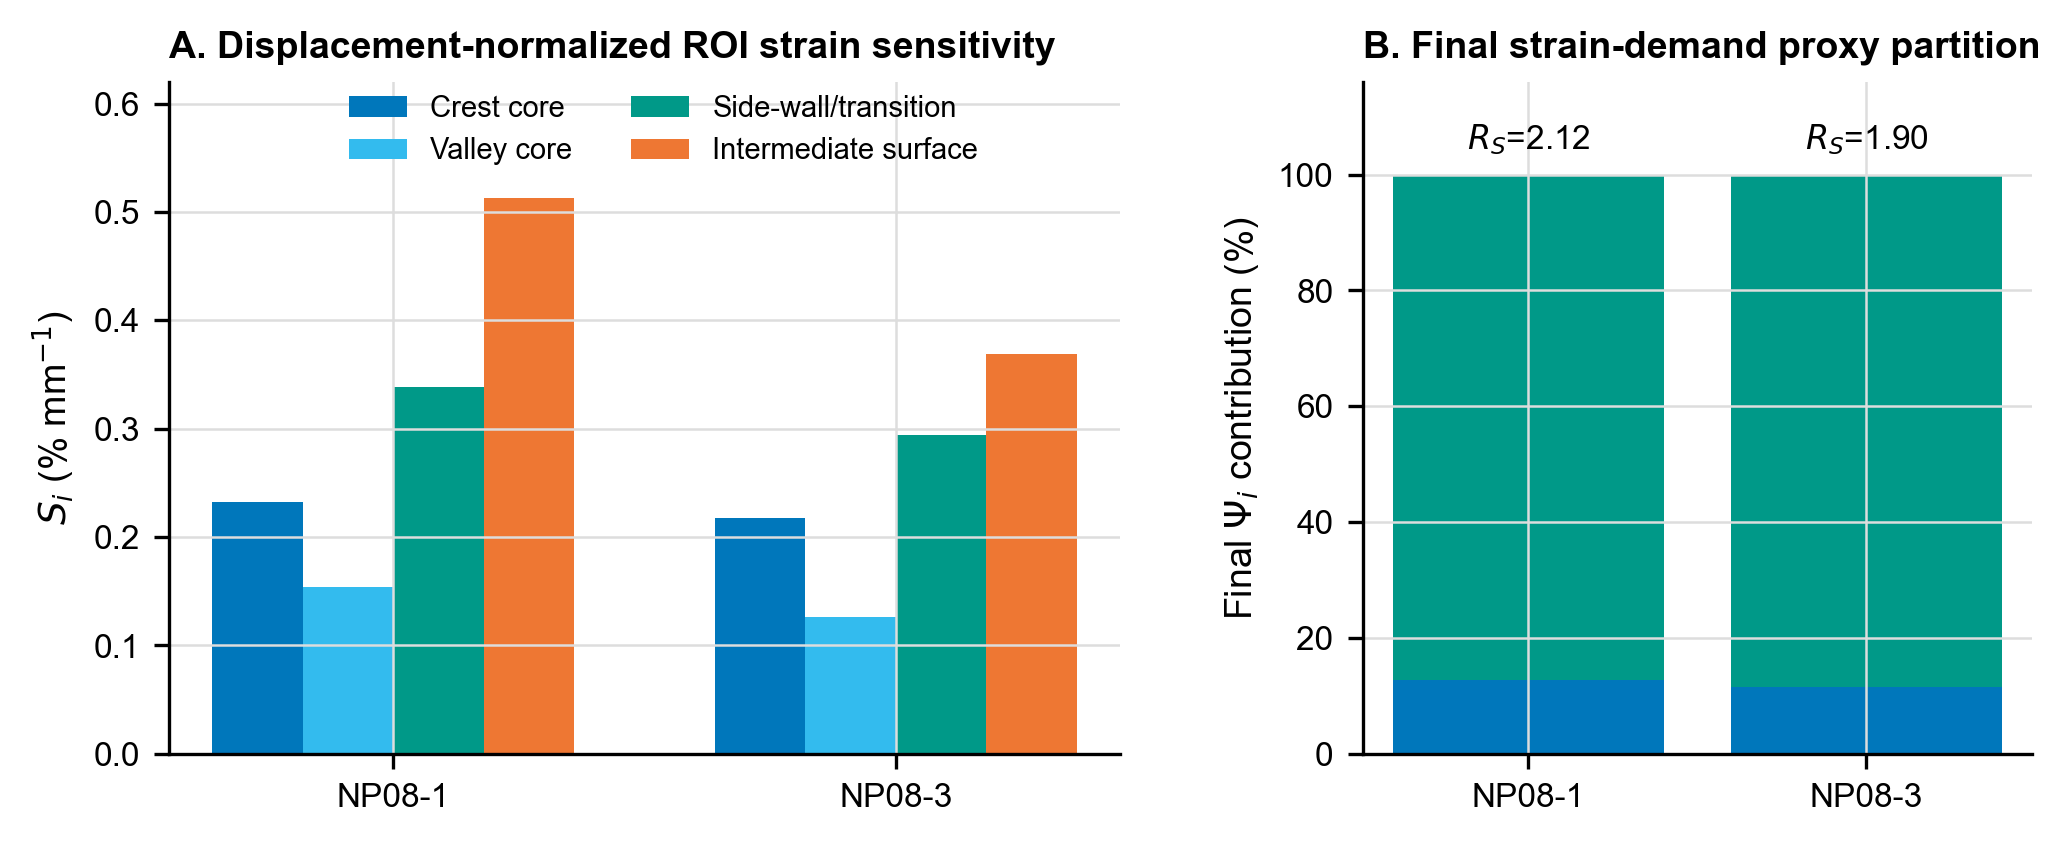
\includegraphics[width=\linewidth,height=14.8cm,keepaspectratio]{assets/fig03_dic_roi_partition.png}
\smallnote{High-deformation ROIs carry most final strain demand.}

\vspace{0.5ex}
\compacttable
\renewcommand{\arraystretch}{1.12}
\begin{tabular}{@{}>{\bfseries}p{0.32\linewidth}>{\centering\arraybackslash}p{0.18\linewidth}>{\centering\arraybackslash}p{0.18\linewidth}p{0.22\linewidth}@{}}
\toprule
Metric & NP08-1 & NP08-3 & Interpretation \\
\midrule
Sensitivity ratio $R_S$ & 2.117 & 1.896 & high-ROI response is about 2x core response \\
High-deformation area & 54.28\% & 53.96\% & deformation path occupies about half the map \\
Final strain-demand share & 87.2\% & 88.4\% & most demand stays in compliant regions \\
\bottomrule
\end{tabular}

\vspace{0.6ex}
\textbf{Mechanism result.} Corrugated specimens show repeated ROI hierarchy: side-wall/transition and intermediate surfaces absorb the imposed displacement while crest/valley cores remain lower-demand regions.
\end{posterblock}
